\subsection{Health and Safety}\label{subsec:healthnsafety}

Since we are working on a pure software project,
we do not interact with any dangerous tools or hardware.
The most fearsome tools for us are actually our office peripherals.
We need to be conscious of the ergonomics of our work environment.


% TODO: add ref, https://www.ccohs.ca/oshanswers/ergonomics/office/monitor_positioning.html
Monitor placement is important because it affects eye strain, and postural strain (neck and shoulders).
It is recommended to keep the monitor approximately forty to seventy cm away from the eyes.
For a quick reference, this is roughly an arm's length away, but it depends on the person.
The monitor height is important as well.
In general, research has found that eyes naturally have a downward cast. % REF.
In fact, they strain more looking above, than looking down.
In practice, guidelines recommend keeping the top of the monitor at eye level, or slightly below.
In general, these are just guidelines to get a good starting point.
It may be worth experimenting depending on the individual's body and what feels best.
A visual summary of these recommendations is given by the Canadian Centre for Occupational Health and Safety (CCOHS) in Figure~\ref{fig:monitor-pos}. % TODO Ref here
\begin{figure}[h]
    \centering
    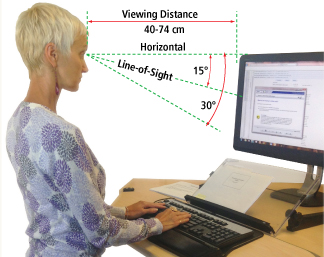
\includegraphics[width=0.5\textwidth]{monitorposition1}
    \caption{The recommended monitor position guidelines from CCOHS.}
    \label{fig:monitor-pos}
\end{figure}

When working for excessively long periods of time without breaks,
it is possible to get repetitive strain injuries (RSI).
It can be from clicking the mouse too much or typing a lot on the keyboard.
Certain mice and keyboards are more ergonomic and help reduce these strains.
They usually have aggressive curves forcing your body to adopt more ergonomic poses.
Office chairs are also an important part of ergonomics, providing proper support while sitting at a desk.

However, even with the best ergonomics setups, the most important is to take frequent breaks from the computer.
Getting up, then walking is good to reduce eye strain, as well as reducing the chances of getting an RSI.
To do this reliably, it is best to set timers and respect them.
Otherwise, there is a risk of getting too absorbed in the work.
After 8 hours of work without breaks writing a report, hands start aching and your body will be the one demanding a break.

% subsection  (end)

\subsection{Engineering Professionalism}\label{subsec:engineering-professionalism}

\subsection{Project Management}\label{subsec:project-management}

